\documentclass[margin=10pt,border=2mm,11pt]{standalone}
\usepackage{tikz}
\usepackage{times}
\usepackage{xcolor}
\usetikzlibrary{shapes.misc,calc,arrows,arrows.meta,patterns,shadings}


 \definecolor{red1}{HTML}{E07A5F}
 \definecolor{blue1}{HTML}{3D405B}
 \definecolor{green1}{HTML}{81B29A}
 \definecolor{orange1}{HTML}{F2CC8F}
 \definecolor{tan1}{HTML}{F4F1DE}
  \definecolor{brightorange1}{HTML}{FCA311}


\newcommand{\cmark}{\ding{51}}%
\newcommand{\xmark}{\ding{55}}%
\newcommand{\smin}{\scalebox{0.9}[0.6]{-}}
\newcommand{\A}{\mathcal{A}}
\begin{document}


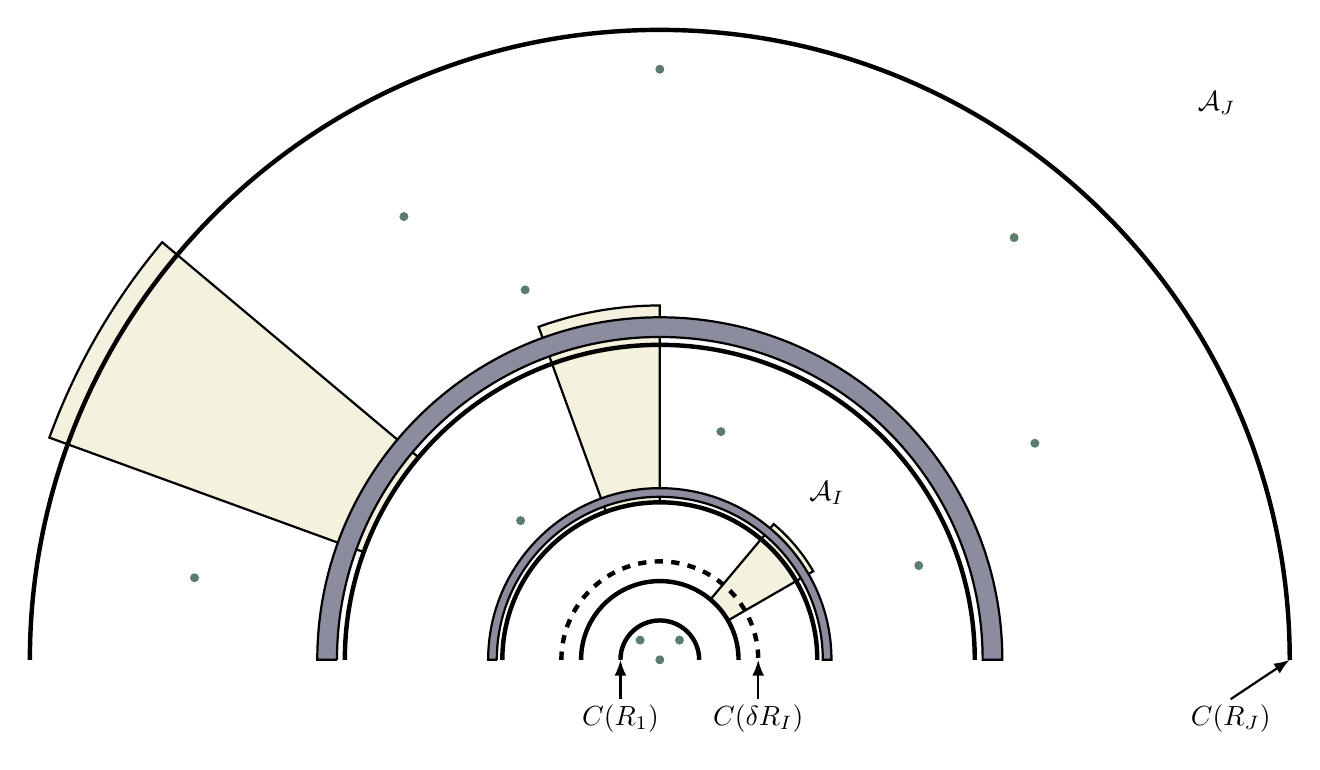
\begin{tikzpicture}




\begin{scope}[scale=1,shift={(0,0)}]

\draw[thick,fill=tan1,fill opacity=1] (160:4) arc (160:140:4) -- (140:8.25) arc (140:160:8.25) -- (160:4);
\draw[thick,fill=tan1,fill opacity=1] (110:2) arc (110:90:2) -- (90:4.5) arc (90:110:4.5) -- (110:2);
\draw[thick,fill=tan1,fill opacity=1] (50:1) arc (50:30:1) -- (30:2.25) arc (30:50:2.25) -- (50:1);

\draw[thick,fill=blue1!60] (180:4.1) arc (180:0:4.1) -- (0:4.35) arc (0:180:4.35) -- (180:4.1);
\draw[thick,fill=blue1!60] (180:2.07) arc (180:0:2.07) -- (0:2.18) arc (0:180:2.18) -- (180:2.07);

\draw[ultra thick] (180:8) arc (180:0:8);
\draw[ultra thick] (180:4) arc (180:0:4);
\draw[ultra thick] (180:2) arc (180:0:2);
\draw[ultra thick] (180:1) arc (180:0:1);
\draw[ultra thick] (180:0.5) arc (180:0:0.5);
\draw[ultra thick,dashed] (180:1.25) arc (180:0:1.25);



\node at (0.25,0.25)[circle, fill=green1!70!black, inner sep=1.15pt]{};
\node at (-0.25,0.25)[circle, fill=green1!70!black, inner sep=1.15pt]{};
\node at (0,0)[circle, fill=green1!70!black, inner sep=1.15pt]{};

\node at (110:5)[circle, fill=green1!70!black, inner sep=1.15pt]{};
\node at (170:6)[circle, fill=green1!70!black, inner sep=1.15pt]{};
\node at (50:7)[circle, fill=green1!70!black, inner sep=1.15pt]{};
\node at (30:5.5)[circle, fill=green1!70!black, inner sep=1.15pt]{};
\node at (90:7.5)[circle, fill=green1!70!black, inner sep=1.15pt]{};
\node at (120:6.5)[circle, fill=green1!70!black, inner sep=1.15pt]{};

\node at (135:2.5)[circle, fill=green1!70!black, inner sep=1.15pt]{};
\node at (75:3)[circle, fill=green1!70!black, inner sep=1.15pt]{};
\node at (20:3.5)[circle, fill=green1!70!black, inner sep=1.15pt]{};



\node at (-0.5,-0.75) {$C( R_1 )$};
\node at (1.25,-0.75) {$C( \delta R_{I} )$};
\node at (7.25,-0.75) {$C( R_{J} )$};

\draw[thick,-{Latex[length=2mm]}] (-0.5,-0.5) -- (-0.5,0);
\draw[thick,-{Latex[length=2mm]}] (1.25,-0.5) -- (1.25,0);
\draw[thick,-{Latex[length=2mm]}] (7.25,-0.5) -- (8,0);

\node at (45:3) {$\A_I$};
\node at (45:10) {$\A_J$};




\end{scope}

\end{tikzpicture}


\end{document}